% % Preamble BEGINN %%%%%%%%%%%%%%%%%%%%%%%%%%%%%%%%%%%%%%%%%%%%%%%%%%%%%%%%%

%%% Preamble (Dokumentenklasse)
% ------------------------------------------------------------------------
% LaTeX - Preambel ******************************************************
% ------------------------------------------------------------------------
% Dokumentklasse (Koma Script)
% ------------------------------------------------------------------------
% basiernd auf www.matthiaspospiech.de/latex/vorlagen Diplomarbeit kompakt
% ========================================================================
\documentclass[%
   %draft,            % Entwurfsstadium
   final,             % fertiges Dokument
   12pt,              % Schriftgroesse der Grundschrift
   bigheadings,       % gro�e �berschriften
   ngerman,           % wird an andere Pakete weitergereicht
   a4paper,           % Papierformat
   BCOR5mm,          % Bindekorrektur: Zus�tzlicher Rand auf der Innenseite
   DIV14,            % Seitengr��e (siehe Koma Skript Dokumentation !)
   1.1headlines,     % Zeilenanzahl der Kopfzeilen
   pagesize,         % Schreibt die Papiergroesse in die Datei.
   oneside,          % Einseitiges Layout
%   twoside,          % Zweiseitiges Layout
   openright,        % Kapitel beginnen immer auf der rechten Seite
   titlepage,        % Titel als einzelne Seite ('titlepage' Umgebung)
   headsepline,      % Linie unter Kolumnentitel ()
%   plainheadsepline, % Linie unter Kolumnentitel () plain Seitenstil
   nochapterprefix,  % keine Ausgabe von 'Kapitel:'
   bibtotoc,         % Bibliographie ins TOC
%	bibtotocnumbered, % Bibliographie ins TOC mit Kapitelnummer
   tocindent,        % eingereuckte Gliederung
   listsindent,      % eingereuckte LOT, LOF
   pointlessnumbers, % Überschriftnummerierung ohne Punkt, siehe DUDEN !
   cleardoubleempty, % Leere linke Seite bei Zweiseitenlayout vor Kapitel
   fleqn,            % Formeln werden linksbuendig angezeigt
%   parindent,        % Absatz mit Einzug (Standard)
   halfparskip,      % Absatz halbe Zeile Abstand
%   parskip,          % Absatz ganze Zeile Abstand
]{scrbook}%     Klassen: scrartcl, scrreprt, scrbook


%%% Alle Namen usw. im Titel und im hyperref-Paket
% ------------------------------------------------------------------------
% LaTeX - Preambel ******************************************************
% ------------------------------------------------------------------------
% pre-work
% ========================================================================
% % ToDo kennzeichnen
\newcommand{\workTodo}[1]{\textcolor{red}{todo: #1}}

% % Für Datum und Zeit in Fusszeile
% % !!!Inhalt bei Fertigstellung der Arbeit löschen
\newcommand{\workMarkDateTime}{}

% % Alle Namen werden im Titel und im hyperref-Paket eingetragen
% % !!! Überall für <Wert> das Entsprechende eintragen

 % <Typ> Studienarbeit, Dipolmarbeit, Studienarbeit oder Bachlor-Abschlussarbeit
\newcommand{\workTyp}{Masterarbeit\xspace}

 % <Titel> der Arbeit
\newcommand{\workTitel}{Map-Matching von Straßeninformationen aus Luftaufnahmen}

 % <Studiengang> z.B. Kommunikationstechnik
\newcommand{\workStudiengang}{Informatik\xspace}

% <Semester> mit Jahr z.B. Sommersemester 2008
\newcommand{\workSemester}{Wintersemester 2018\xspace}

% <Name> des Studenten
\newcommand{\workNameStudent}{Steffen Schmid\xspace}

% <Pruefer> Name des pr�fenden (betreuenden) Professor an der Hochschule
\newcommand{\workPruefer}{Prof. Dr. Christoph Reich\xspace}


% %%% Nur bei Abschluss-Arbeiten

% <Datum> der Abgabe der Arbeit (Eidesstatliche Erklärung)
\newcommand{\workDatum}{\today\xspace}

% <Zweitpr�fer>
\newcommand{\workZweitPruefer}{}

% <Zeitraum>
\newcommand{\workZeitraum}{13.02.2017 - 11.08.2017\xspace}


% %%% Nur bei Industrie-Arbeiten:

% <Firma>
\newcommand{\workFirma}{IT-Designers GmbH\xspace}

% <Betreuer in der Firma>
\newcommand{\workBetreuer}{Stefan Kaufmann\xspace}

%%% Preamble (Pakete)
% ------------------------------------------------------------------------
% LaTeX - Preambel ******************************************************
% ------------------------------------------------------------------------
% Packages
% ------------------------------------------------------------------------
% basiernd auf www.matthiaspospiech.de/latex/vorlagen Diplomarbeit kompakt
% ========================================================================

% Inhalt:
% 1. Einige Pakete muessen unbedingt vor allen anderen geladen werden
% 2. Fonts Fonts Fonts
% 3. Math Packages
% 4. Symbole
% 5. text related packages
% 6. Pakete zum Zitieren
% 7. PDF related packages
% 8. Tables (Tabular)
% 9. figures and placement
% 10. verbatim packages
% 11. science packages
% 12. layout packages

% ~~~~~~~~~~~~~~~~~~~~~~~~~~~~~~~~~~~~~~~~~~~~~~~~~~~~~~~~~~~~~~~~~~~~~~~~
% Encoding der Dateien (sonst funktionieren Umlaute nicht)
% Empfohlen latin1, da einige Pakete mit utf8 Zeichen nicht
% funktionieren, z.B: listings, soul.

% \usepackage[latin1]{inputenx} % ISO-8859-1
% \usepackage[ansinew]{inputenx} % Windows-Standard (CP1252) (baut auf ISO 8859-1 und ISO 8859-15 auf)
\usepackage[utf8]{inputenc}

% ~~~~~~~~~~~~~~~~~~~~~~~~~~~~~~~~~~~~~~~~~~~~~~~~~~~~~~~~~~~~~~~~~~~~~~~~
% 1. Einige Pakete muessen unbedingt vor allen anderen geladen werden
% ~~~~~~~~~~~~~~~~~~~~~~~~~~~~~~~~~~~~~~~~~~~~~~~~~~~~~~~~~~~~~~~~~~~~~~~~
%
\usepackage{xspace} % Define commands that don't eat spaces.
\usepackage{ifpdf} % Fuer Pakete/Paketoptionen, die nur fuer pdf benoetigt werden \ifpdf \else \fi
\usepackage{calc} % Calculation with LaTeX
\usepackage[ngerman]{babel} % Languagesetting
\usepackage[table]{xcolor} % Farben
\usepackage[]{graphicx} % Bilder
%\usepackage{epstopdf} % If an eps image is detected, epstopdf is automatically called to convert it to pdf format.
\usepackage[]{amsmath} % Amsmath - Mathematik Basispaket
\usepackage{ragged2e} % Besserer Flatternsatz (Linksbuendig, statt Blocksatz)

% ~~~~~~~~~~~~~~~~~~~~~~~~~~~~~~~~~~~~~~~~~~~~~~~~~~~~~~~~~~~~~~~~~~~~~~~~
% 2. Fonts Fonts Fonts
% ~~~~~~~~~~~~~~~~~~~~~~~~~~~~~~~~~~~~~~~~~~~~~~~~~~~~~~~~~~~~~~~~~~~~~~~~

\usepackage[T1]{fontenc} % T1 Schrift Encoding (notwendig f�r die meisten Type 1 Schriften)
\usepackage{textcomp}	 % Zusatzliche Symbole (Text Companion font extension)

% Alle Schriften die hier angegeben sind sehen im PDF richtig aus.
% Die LaTeX Standardschrift ist die Latin Modern (lmodern Paket).
% If Latin Modern is not available for your distribution you must install the
% package cm-super instead. Otherwise your fonts will look horrible in the PDF

% DO NOT LOAD ae-Package for the font !

%% - Latin Modern
\usepackage{lmodern}
%% -------------------
%
% % - Times, Helvetica, Courier (Word Standard...)
%\usepackage{mathptmx}
%\usepackage[scaled=.90]{helvet}
%\usepackage{courier}
% % -------------------
%%
%% - Palantino , Helvetica, Courier
%\usepackage{mathpazo}
%\usepackage[scaled=.95]{helvet}
%\usepackage{courier}
%% -------------------
%
%% - Bera Schriften
%\usepackage{bera}
%% -------------------
%
%% - Charter, Bera Sans
%\usepackage{charter}\linespread{1.05}
%\renewcommand{\sfdefault}{fvs}


% ~~~~~~~~~~~~~~~~~~~~~~~~~~~~~~~~~~~~~~~~~~~~~~~~~~~~~~~~~~~~~~~~~~~~~~~~
% 3. Math Packages
% ~~~~~~~~~~~~~~~~~~~~~~~~~~~~~~~~~~~~~~~~~~~~~~~~~~~~~~~~~~~~~~~~~~~~~~~~

\usepackage[fixamsmath,disallowspaces]{mathtools} % Erweitert amsmath und behebt einige Bugs
\usepackage{fixmath}
\usepackage[all,warning]{onlyamsmath} % Warnt bei Benutzung von Befehlen die mit amsmath inkompatibel sind.
\usepackage{icomma} % Erlaubt die Benutzung von Kommas im Mathematikmodus

% ~~~~~~~~~~~~~~~~~~~~~~~~~~~~~~~~~~~~~~~~~~~~~~~~~~~~~~~~~~~~~~~~~~~~~~~~
% 4. Symbole
% ~~~~~~~~~~~~~~~~~~~~~~~~~~~~~~~~~~~~~~~~~~~~~~~~~~~~~~~~~~~~~~~~~~~~~~~~
\usepackage{amssymb}
%\usepackage{wasysym}
%\usepackage{marvosym}
%\usepackage{pifont}

% ~~~~~~~~~~~~~~~~~~~~~~~~~~~~~~~~~~~~~~~~~~~~~~~~~~~~~~~~~~~~~~~~~~~~~~~~
% 5. text related packages
% ~~~~~~~~~~~~~~~~~~~~~~~~~~~~~~~~~~~~~~~~~~~~~~~~~~~~~~~~~~~~~~~~~~~~~~~~

\usepackage{url} % Setzen von URLs. In Verbindung mit hyperref sind diese auch aktive Links.
\usepackage[stable,perpage, ragged,  multiple]{footmisc} % Fussnoten
\usepackage[ngerman]{varioref} % Intelligente Querverweise
\usepackage{enumitem} % Listen

% ~~~~~~~~~~~~~~~~~~~~~~~~~~~~~~~~~~~~~~~~~~~~~~~~~~~~~~~~~~~~~~~~~~~~~~~~
% 6. Pakete zum Zitieren
% ~~~~~~~~~~~~~~~~~~~~~~~~~~~~~~~~~~~~~~~~~~~~~~~~~~~~~~~~~~~~~~~~~~~~~~~~

\usepackage[babel, german=quotes, english=british, french=guillemets]{csquotes} % clever quotations
\SetBlockThreshold{2} % Anzahl von Zeilen
\newenvironment{myquote}%
          {\begin{quote}\small}%
          {\end{quote}}%
\SetBlockEnvironment{myquote}

% \usepackage[backend=biber]{biblatex}
\usepackage[square]{natbib}
\bibliographystyle{dinat}
    
% ~~~~~~~~~~~~~~~~~~~~~~~~~~~~~~~~~~~~~~~~~~~~~~~~~~~~~~~~~~~~~~~~~~~~~~~~
% 7. PDF related packages
% ~~~~~~~~~~~~~~~~~~~~~~~~~~~~~~~~~~~~~~~~~~~~~~~~~~~~~~~~~~~~~~~~~~~~~~~~

\ifpdf % Wenn als PDF ausgegeben wird
\usepackage{pdfpages} % pdf-Seiten einbinden
\usepackage[pdftex]{hyperref} % PDF Option in Hyperref
\else
\usepackage[dvipdfm]{hyperref}
\fi

%%% Doc: ftp://tug.ctan.org/pub/tex-archive/macros/latex/contrib/pdfpages/pdfpages.pdf
%\usepackage{pdfpages} % Include pages from external PDF documents in LaTeX documents

%%% Doc: ftp://tug.ctan.org/pub/tex-archive/macros/latex/contrib/hyperref/doc/manual.pdf
\hypersetup{
          pdfhighlight = /O,	         % Visualisierung beim anklicken von Links
% Farben fuer die Links
   colorlinks=true,	        % Links erhalten Farben statt Kaestchen
   urlcolor=black,    % \href{...}{...} external (URL)
   filecolor=black,  % \href{...} local file
   linkcolor=black,  % \ref{...} and \pageref{...}
   citecolor =black,    % Literaturverzeichnis
   % Links
   raiselinks=true,			 % calculate real height of the link
   breaklinks,	        % Links bestehen bei Zeilenumbruch
%   backref=page,	         % Backlinks im Literaturverzeichnis (section, slide, page, none)
%   pagebackref=true,        % Backlinks im Literaturverzeichnis mit Seitenangabe
   verbose,
%   hyperindex=true,         % backlinkex index
   linktocpage=true,        % Inhaltsverzeichnis verlinkt Seiten
%   hyperfootnotes=false,	% Keine Links auf Fussnoten
   % Bookmarks
%   bookmarks=true,	         % Erzeugung von Bookmarks fuer PDF-Viewer
   bookmarksopenlevel=1,    % Gliederungstiefe der Bookmarks
   bookmarksopen=true,      % Expandierte Untermenues in Bookmarks
   bookmarksnumbered=true,  % Nummerierung der Bookmarks
   bookmarkstype=toc,       % Art der Verzeichnisses
   % Anchors
   plainpages=false,        % % Make page anchors using the formatted form of the page number. With this option, hyperref writes different anchors for pages �ii� and �2�. (If the option is set �true� � the default � hyperref writes page anchors as the arabic form of the absolute page number, rather than the formatted form.)
   % hypertexnames=false,
   pageanchor=true,	        % Pages are linkable
   % PDF Informationen
   pdftitle={\workTyp: \workTitel},	        % Titel
   pdfauthor={\workNameStudent},	    % Autor
   pdfcreator={LaTeX, hyperref, KOMA-Script}, % Ersteller
   %pdfproducer={pdfeTeX 1.10b-2.1} %Produzent
   pdfstartview=FitH,       % Dokument wird Fit Width geaefnet
   pdfpagemode=UseOutlines, % Bookmarks im Viewer anzeigen
%   pdfpagelabels=true,      % set PDF page labels
}

% ~~~~~~~~~~~~~~~~~~~~~~~~~~~~~~~~~~~~~~~~~~~~~~~~~~~~~~~~~~~~~~~~~~~~~~~~
% 8. Tables (Tabular)
% ~~~~~~~~~~~~~~~~~~~~~~~~~~~~~~~~~~~~~~~~~~~~~~~~~~~~~~~~~~~~~~~~~~~~~~~~

\usepackage{booktabs}
\usepackage{tabularx} % tabularx nach hyperref laden
\usepackage{multirow}

\usepackage{scrextend}
% \addtokomafont{labelinglabel}

% ~~~~~~~~~~~~~~~~~~~~~~~~~~~~~~~~~~~~~~~~~~~~~~~~~~~~~~~~~~~~~~~~~~~~~~~~
% 9. figures and placement
% ~~~~~~~~~~~~~~~~~~~~~~~~~~~~~~~~~~~~~~~~~~~~~~~~~~~~~~~~~~~~~~~~~~~~~~~~

%% Bilder und Graphiken ==================================================

\usepackage{float}	% Stellt die Option [H] fuer Floats zur Verfgung
\usepackage{flafter} % Floats immer erst nach der Referenz setzen
\usepackage{subfig} % Layout wird weiter unten festgelegt !
\usepackage{wrapfig} % Bilder von Text Umfliessen lassen
\usepackage{svg}

\usepackage{placeins} % Alle Floats bis \FloatBarrier ausgeben

% Make float placement easier
\renewcommand{\floatpagefraction}{.75} % vorher: .5
\renewcommand{\textfraction}{.1}       % vorher: .2
\renewcommand{\topfraction}{.8}        % vorher: .7
\renewcommand{\bottomfraction}{.5}     % vorher: .3
\setcounter{topnumber}{3}	         % vorher: 2
\setcounter{bottomnumber}{2}	         % vorher: 1
\setcounter{totalnumber}{5}	         % vorher: 3


% ~~~~~~~~~~~~~~~~~~~~~~~~~~~~~~~~~~~~~~~~~~~~~~~~~~~~~~~~~~~~~~~~~~~~~~~~
% 10. verbatim packages
% ~~~~~~~~~~~~~~~~~~~~~~~~~~~~~~~~~~~~~~~~~~~~~~~~~~~~~~~~~~~~~~~~~~~~~~~~

%%% Doc: ftp://tug.ctan.org/pub/tex-archive/macros/latex/contrib/upquote/upquote.sty
\usepackage{upquote} % Setzt "richtige" Quotes in verbatim-Umgebung

%%% Doc: No Documentation
% \usepackage{verbatim} % Reimplemntation of the original verbatim

%%% Doc: http://www.cs.brown.edu/system/software/latex/doc/fancyvrb.pdf
% \usepackage{fancyvrb} % Superior Verbatim Class

%% Listings Paket ------------------------------------------------------
%%% Doc: ftp://tug.ctan.org/pub/tex-archive/macros/latex/contrib/listings/listings-1.3.pdf
\usepackage{listings}
% \usepackage{minted}

\lstset{
basicstyle =\ttfamily\color{black}\small, % Standardschrift
keywordstyle =, % \bfseries\color{blue}	  % Schl�sselwort-Style
%identifierstyle =\underbar,
commentstyle =\color{teal},
stringstyle =\itshape,
numbers = left,			  % Ort der Zeilennummern
numberstyle =\tiny\color{black},	   % Stil der Zeilennummern
numbers = left,			  % Ort der Zeilennummern
tabsize=2,			  % Groesse von Tabs
breaklines,			  % Zeilen werden Umgebrochen
breakatwhitespace,			  % An Leerzeichen umbrechen
%showspaces=true,			  % Leerzeichen anzeigen
backgroundcolor=\color[RGB]{242, 242, 242},	  % % Hintergrundfarbe der Listings
}
 \lstloadlanguages{
         [AlLaTeX]TeX,
         C++
 }

 \lstset{language=C++,
                 basicstyle=\ttfamily,
                 keywordstyle=\color{blue}\ttfamily,
                 stringstyle=\color{red}\ttfamily,
                 commentstyle=\color{green}\ttfamily,
                 morecomment=[l][\color{magenta}]{\#}
 }

\definecolor{bluekeywords}{rgb}{0.13,0.13,1}
\definecolor{greencomments}{rgb}{0,0.5,0}
\definecolor{redstrings}{rgb}{0.9,0,0}

\lstdefinelanguage{FSharp}%
{morekeywords={let, new, match, with, rec, open, module, namespace, type, alias of, member, %
and, for, while, true, false, in, do, begin, end, fun, function, return, yield, try, %
mutable, if, then, else, cloud, async, static, use, abstract, interface, inherit, finally, default },
  otherkeywords={ let!, return!, do!, yield!, use!, var, from, select, where, order, by },
  keywordstyle=\color{bluekeywords},
  sensitive=true,
  basicstyle=\ttfamily,
  breaklines=true,
  xleftmargin=\parindent,
  aboveskip=\bigskipamount,
  tabsize=4,
  morecomment=[l][\color{greencomments}]{///},
  morecomment=[l][\color{greencomments}]{//},
  morecomment=[s][\color{greencomments}]{{(*}{*)}},
  morestring=[b]",
  showstringspaces=false,
  literate={`}{\`}1,
  stringstyle=\color{redstrings},
}

% \usepackage{elm-highlighting}

%%% Doc: ftp://tug.ctan.org/pub/tex-archive/macros/latex/contrib/examplep/eurotex_2005_examplep.pdf
% LaTeX Code und Ergebnis nebeneinander darstellen
%\usepackage{examplep}

\usepackage[acronym, toc, nopostdot, xindy, style=super]{glossaries}

% ~~~~~~~~~~~~~~~~~~~~~~~~~~~~~~~~~~~~~~~~~~~~~~~~~~~~~~~~~~~~~~~~~~~~~~~~
% 11. science packages
% ~~~~~~~~~~~~~~~~~~~~~~~~~~~~~~~~~~~~~~~~~~~~~~~~~~~~~~~~~~~~~~~~~~~~~~~~

\usepackage[squaren]{SIunits}

% ~~~~~~~~~~~~~~~~~~~~~~~~~~~~~~~~~~~~~~~~~~~~~~~~~~~~~~~~~~~~~~~~~~~~~~~~
% 12. layout packages
% ~~~~~~~~~~~~~~~~~~~~~~~~~~~~~~~~~~~~~~~~~~~~~~~~~~~~~~~~~~~~~~~~~~~~~~~~

%% Zeilenabstand =========================================================
%
%%% Doc: ftp://tug.ctan.org/pub/tex-archive/macros/latex/contrib/setspace/setspace.sty
\usepackage{setspace}
%\doublespace	        % 2-facher Abstand
%\onehalfspace	  % 1,5-facher Abstand
% hereafter load 'typearea' again

%% Seitenlayout ==========================================================
%
% Layout mit 'typearea'
\typearea[current]{last}
\raggedbottom     % Variable Seitenhoehen zulassen


%% Kopf und Fusszeilen====================================================
%%% Doc: ftp://tug.ctan.org/pub/tex-archive/macros/latex/contrib/koma-script/scrguide.pdf
\usepackage[%
   automark,	 % automatische Aktualisierung der Kolumnentitel
   nouppercase,	 % Grossbuchstaben verhindern
]{scrpage2}

\usepackage{scrtime} % Zeit
%\usepackage{scrdate} % Datum

\pagestyle{scrheadings} % Seite mit Headern
%\pagestyle{scrplain} % Seiten ohne Header
%\pagestyle{empty} % Seiten ohne Header

% loescht voreingestellte Stile
\clearscrheadings
\clearscrplain
%
% [scrplain]{scrheadings}

% %%% Kopfzeile
% einseitig: Bei einseitigem Layout, nur folgende Zeilen verwenden !!!
\ihead[]{\leftmark} % links: Kapitel
 %\chead[\pagemark]{\pagemark} % mitte:
\ohead[]{\rightmark} % rechts: Section

% %zweiseitig: Bei zweiseitigem Layout, nur folgende Zeilen verwenden !!!
%\ihead[]{} % innen
% % \chead[\pagemark]{\pagemark} % mitte:
%\ohead[]{\headmark} % aussen: Kapitel (linke Seite) und Section (rechte Seite)
%
% %%% Fusszeile
\ifoot[\workMarkDateTime]{\workMarkDateTime} % innen:
%\cfoot[\pagemark]{\pagemark} % mitte:
\ofoot[\pagemark]{\pagemark} % aussen: Seitenzahl

% Angezeigte Abschnitte im Header
\automark[section]{chapter} % Inhalt von [\rightmark]{\leftmark}
%
% Linie zwischen Kopf und Textk�rper
\setheadsepline{.4pt}[\color{black}]

%% Fussnoten =============================================================
% Keine hochgestellten Ziffern in der Fussnote (KOMA-Script-spezifisch):
\deffootnote{1.5em}{1em}{\makebox[1.5em][l]{\thefootnotemark}}
\addtolength{\skip\footins}{\baselineskip} % Abstand Text <-> Fussnote
\setlength{\dimen\footins}{10\baselineskip} % Beschraenkt den Platz von Fussnoten auf 10 Zeilen
\interfootnotelinepenalty=10000 % Verhindert das Fortsetzen von
                                % Fussnoten auf der gegen�berligenden Seite

%% Schriften (Sections )==================================================

% -- Koma Schriften --
\newcommand\SectionFontStyle{\sffamily}

\setkomafont{chapter}{\huge\SectionFontStyle}    % Chapter
\setkomafont{sectioning}{\SectionFontStyle} %  % Titelzeilen % \bfseries

\setkomafont{pagenumber}{\bfseries\SectionFontStyle} % Seitenzahl
\setkomafont{pagehead}{\small\sffamily}	       % Kopfzeile

\setkomafont{descriptionlabel}{\itshape}        % Stichwortliste
%
\renewcommand*{\raggedsection}{\raggedright} % Titelzeile linksbuendig, haengend
%

%% Captions (Schrift, Aussehen) ==========================================

%%% Doc: ftp://tug.ctan.org/pub/tex-archive/macros/latex/contrib/caption/caption.pdf
\usepackage{caption}
% Aussehen der Captions
\captionsetup{
   margin = 10pt,
   font = {small,rm},
   labelfont = {small,bf},
   format = plain, % oder 'hang'
   indention = 0em,	 % Einruecken der Beschriftung
   labelsep = colon, %period, space, quad, newline
   justification = RaggedRight, % justified, centering
   singlelinecheck = true, % false (true=bei einer Zeile immer zentrieren)
   position = bottom %top
}
%%% Bugfix Workaround
\DeclareCaptionOption{parskip}[]{}
\DeclareCaptionOption{parindent}[]{}

% Aussehen der Captions fuer subfigures (subfig-Paket)
\captionsetup[subfloat]{%
   margin = 10pt,
   font = {small,rm},
   labelfont = {small,bf},
   format = plain, % oder 'hang'
   indention = 0em,	 % Einruecken der Beschriftung
   labelsep = space, %period, space, quad, newline
   justification = RaggedRight, % justified, centering
   singlelinecheck = true, % false (true=bei einer Zeile immer zentrieren)
   position = bottom, %top
   labelformat = parens % simple, empty % Wie die Bezeichnung gesetzt wird
 }

%% Inhaltsverzeichnis (Schrift, Aussehen) sowie weitere Verzeichnisse ====

\setcounter{secnumdepth}{2}	 % Abbildungsnummerierung mit groesserer Tiefe
\setcounter{tocdepth}{2}		 % Inhaltsverzeichnis mit groesserer Tiefe
%

% Farben ================================================================
% Farben fuer die Links im PDF

\definecolor{green}{rgb}{0,0.5,0} % gr�n
\definecolor{brown}{rgb}{0.6,0,0} % braun
\definecolor{darkblue}{rgb}{0,0,.5} % dunkelblau
\definecolor{lightblue}{rgb}{0.8,0.85,1} % hellblau
% Farben fuer Listings
\colorlet{stringcolor}{green!40!black!100}
\colorlet{commencolor}{blue!0!black!100}


% Auszufuehrende Befehle  ------------------------------------------------

%\listfiles
%------------------------------------------------------------------------


\loadglsentries{glossaries}
\glossarystyle{super}
\makeglossaries

%%% Neue Befehle
% ------------------------------------------------------------------------
% LaTeX - Preambel ******************************************************
% ------------------------------------------------------------------------
% pre-newcommands
% ========================================================================
% ---- Hervorhebungen
% demo.tex Hervorhebungen
\newcommand{\env}[1]{\texttt{#1}}
\newcommand{\command}[1]{\texttt{#1}}
\newcommand{\package}[1]{\texttt{\itshape#1}}
\newcommand{\engl}[1]{(engl: \textit{#1})\xspace}

% todo
% \newcommand{\todo}[1]{{\color{red}#1}\xspace}
\newcommand{\bv}{\todo{BV}} % Begriffsverzeichnis
\newcommand{\kap}{\todo{Kp}} % Kapitel

% TeX
\newcommand{\latex}{\LaTeX\xspace}
\newcommand{\tex}{\TeX\xspace}
\newcommand{\miktex}{MiK\TeX\xspace}
\newcommand{\bibtex}{Bib\TeX\xspace}

\newcommand{\led}{LEd\xspace}

\newcommand{\koma}{KOMA-Script\xspace}

% Internetseite
\newcommand{\www}[1]{\href{http://#1}{#1}}
\newcommand{\wwwhttp}[1]{\href{#1}{#1}}
\newcommand{\wwwlink}[1]{\footnote{\www{#1}}}

% Textauszeichnungen
\newcommand{\textemph}[1]{\textit{#1}} % Hervorheben
\newcommand{\textemphs}[1]{\textbf{#1}} % Hervorheben fett
\newcommand{\textqu}[1]{\enquote{#1}} % Anf�hrungszeichen
\newcommand{\tshortcut}[1]{\textit{#1}}
\newcommand{\textbutton}[1]{\textit{#1}}
\newcommand{\textmenu}[1]{\textit{#1}}
\newcommand{\textlst}[1]{\texttt{#1}} % Listings im Text
%\newcommand{\textcode}[1]{\texttt{#1}\xspace} %
%\newcommand{\texttask}[1]{\textit{#1}}


% ---- Abkuerzungen
\newcommand{\zB}{\mbox{z.\,B.}\xspace}
\newcommand{\ua}{\mbox{u.\,a.}\xspace}
\newcommand{\dah}{\mbox{d.\,h.}\xspace}
\newcommand{\uAe}{\mbox{u.\,�.}\xspace}

% ---- Listings
\newcommand{\lst}[1]{\lstinline$#1$} % geht nicht

\newcommand{\lstergibt}[1]{Ergibt:\newline{}}
%%%%%%%%%%%%%%%%%%%%%%%%%%%%%%%%%%%%%%%%%%%%%%%%%%%%%%%%%%%%%%%%%%%%%%%%%%%%%%
% ---- Querverweise
\newcommand{\refs}[1]{\mbox{(s.~\autoref{#1})}\xspace}
\newcommand{\refsauch}[1]{(s. auch \autoref{#1})\xspace}
\newcommand{\refn}[1]{\mbox{\autoref{#1}\xspace}} % normal

\newcommand{\refnp}[1]{\mbox{(\autopageref{#1})}\xspace}
\newcommand{\refp}[1]{Seite~\pageref{#1}\xspace}
%
\newcommand{\refk}[1]{Kapitel~\ref{#1}\xspace}
\newcommand{\refa}[1]{Abbildung~\ref{#1}\xspace}
\newcommand{\reft}[1]{Tabelle~\ref{#1}\xspace}
\newcommand{\reflst}[1]{Listing~\ref{#1}\xspace}
%%%%%%%%%%%%%%%%%%%%%%%%%%%%%%%%%%%%%%%%%%%%%%%%%%%%%%%%%%%%%%%%%%%%%%%%%%%%%%
% % ---- Literatur
% Verweise
% \newcommand{\cites}[2]{(s. \cite[#1]{#2})\xspace}

% Bild aus Literaturv.
\newcommand{\cbild}[1]{(Bild~\cite{#1})\xspace}
%

%%%%%%%%%%%%%%%%%%%%%%%%%%%%%%%%%%%%%%%%%%%%%%%%%%%%%%%%%%%%%%%%%%%%%%%%%%%%%%
% ---- Namen der Links im Dokument
% ngerman (Babel-Paket) Namen umbenennen
\addto\captionsngerman{\renewcommand\figurename{Abbildung}}
\addto\captionsngerman{\renewcommand\tablename{Tabelle}}
\addto\captionsngerman{\renewcommand\lstlistingname{Listing}}
%
%\addto\captionsngerman{\renewcommand\contentsname{Inhalt}}
%\addto\captionsngerman{\renewcommand\appendixname{Anhang}}
%\addto\captionsngerman{\renewcommand\lstlistlistingname{Listings}}
%
%\addto\extrasngerman{\def\partautorefname{Teil}}
\addto\extrasngerman{\def\chapterautorefname{Kap.}}
\addto\extrasngerman{\def\sectionautorefname{Kap.}}
\addto\extrasngerman{\def\subsectionautorefname{Kap.}}
\addto\extrasngerman{\def\subsubsectionautorefname{Kap.}}
\addto\extrasngerman{\def\subsectionautorefname{Kap.}}
\addto\extrasngerman{\def\paragraphautorefname{Kap.}}
\addto\extrasngerman{\def\subparagraphautorefname{Kap.}}
\addto\extrasngerman{\def\appendixautorefname{Kap.}}
%
\addto\extrasngerman{\def\figureautorefname{Abb.}}
\addto\extrasngerman{\def\tableautorefname{Tab.}}
\addto\extrasngerman{\def\equationautorefname{Gl.}}
\addto\extrasngerman{\def\theoremautorefname{Gl.}}
\addto\extrasngerman{\def\AMSnameautorefname{Gl.}}
\addto\extrasngerman{\def\pageautorefname{S.}}
%
%\addto\extrasngerman{\def\itemautorefname{Pkt.}}
%\addto\extrasngerman{\def\Hfootnoteautorefname{Fu�note}}
\addto\extrasngerman{\def\lstlistingautorefname{List.}}

% ------------------------------------------------------------------------
% LaTeX - Preambel ******************************************************
% ------------------------------------------------------------------------
% Table Commands
% ------------------------------------------------------------------------
% basiernd auf www.matthiaspospiech.de/latex/vorlagen Diplomarbeit kompakt
% ========================================================================
%% Kommandos fuer Tabellen. Entnommen aus The LateX Companion, tabsatz.ps und diversen Dokus

%%% ---| Farben fuer Tabellen |-------------------
\colorlet{tablesubheadcolor}{gray!30}
\colorlet{tableheadcolor}{gray!25}
\colorlet{tableblackheadcolor}{black!100}
\colorlet{tablerowcolor}{gray!10.0}
%%% ---------------------------------------------

% um Tabellenspalten mit Flattersatz zu setzen, muss \\ vor
% (z.B.) \raggedright geschuetzt werden:
\newcommand{\PreserveBackslash}[1]{\let\temp=\\#1\let\\=\temp}

% Linksbuendig:
\newcolumntype{v}[1]{>{\PreserveBackslash\RaggedRight\hspace{0pt}}p{#1}}
\newcolumntype{M}[1]{>{\PreserveBackslash\RaggedRight\hspace{0pt}}m{#1}}
\newcolumntype{Y}{>{\PreserveBackslash\RaggedLeft\hspace{0pt}}X}

\newcolumntype{Z}{>{\PreserveBackslash\RaggedRight\hspace{0pt}}X}

%%% ---|Layout der Tabellen |-------------------


% Groesse der Schrift in Tabellen
\newcommand{\tablefontsize}{ \footnotesize}
\newcommand{\tableheadfontsize}{\footnotesize}

% Layout der Tabelle: Ausrichtung, Schrift, Zeilenabstand
\newcommand\tablestylecommon{%
  \renewcommand{\arraystretch}{1.4} % Groessere Abstaende zwischen Zeilen
  \normalfont\normalsize            %
  \sffamily\tablefontsize           % Serifenlose und kleine Schrift
  \centering%                       % Tabelle zentrieren
}

\newcommand{\tablestyle}{
	\tablestylecommon
	%\tablealtcolored
}

% Ruecksetzten der Aenderungen
\newcommand\tablerestoresettings{%
  \renewcommand{\arraystretch}{1}% Abstaende wieder zuruecksetzen
  \normalsize\rmfamily % Schrift wieder zuruecksetzen
}

% % Tabellenkopf: Serifenlos+fett+schraeg+Schriftfarbe
% \newcommand\tablehead{%
%   \tableheadfontsize%
%   \sffamily\bfseries%
%   %\slshape
%   %\color{white}
% }

\newcommand\tablesubheadfont{%
  \tableheadfontsize%
  \sffamily\bfseries%
  \slshape
  %\color{white}
}


\newcommand\tableheadcolor{%
	%\rowcolor{tablesubheadcolor}
	%\rowcolor{tableblackheadcolor}
	\rowcolor{tableheadcolor}%
}

\newcommand\tablesubheadcolor{%
	\rowcolor{tablesubheadcolor}
	%\rowcolor{tableblackheadcolor}
}

\newcommand{\tableend}{\arrayrulecolor{black}\hline}


\newcommand{\tablesubhead}[2]{%
  \multicolumn{#1}{>{\columncolor{tablesubheadcolor}}l}{\tablesubheadfont #2}%
}

% Tabellenbody (=Inhalt)
\newcommand\tablebody{%
\tablefontsize\sffamily\upshape%
}

\newcommand\tableheadshaded{%
	\rowcolor{tableheadcolor}%
}
\newcommand\tablealtcolored{%
	\rowcolors{1}{tablerowcolor}{white!100}%
}
%%% --------------------------------------------
 % Fuer Tabellen

%%% Silbentrennung
% ------------------------------------------------------------------------
% LaTeX - Preambel ******************************************************
% ------------------------------------------------------------------------
% pre-hyphenation
% ========================================================================
\hyphenation{Koordi-naten}
\hyphenation{Un-super-vised-Tracking}
 


% % Preamble ENDE %%%%%%%%%%%%%%%%%%%%%%%%%%%%%%%%%%%%%%%%%%%%%%%%%%%%%%%%%%

% % Inhalt BEGINN %%%%%%%%%%%%%%%%%%%%%%%%%%%%%%%%%%%%%%%%%%%%%%%%%%%%%%%%%
\begin{document}
% Tabellen-Einstellungen
% ------------------------------------------------------------------------
% LaTeX - (Preambel) *****************************************************
% ------------------------------------------------------------------------
% Table Settings
% ------------------------------------------------------------------------
% basiernd auf www.matthiaspospiech.de/latex/vorlagen Diplomarbeit kompakt
% ========================================================================
% Einstellungen f�r Tabellen

\renewcommand\tablestylecommon{%
  \renewcommand{\arraystretch}{1.4} % Groessere Abstaende zwischen Zeilen
  \normalfont\normalsize            %
  \sffamily\tablefontsize           % Serifenlose und kleine Schrift
  \centering%                       % Tabelle zentrieren
}

\renewcommand{\tablestyle}{%
   \tablestylecommon%
}

\renewcommand\tablebody{%
   \tablefontsize\sffamily\upshape%
}

% % %%%%%% Vorspiel
\begin{spacing}{1} % Vorspiel immer mit Standard-Zeilenabstand setzen
	\frontmatter
	% % Titelblatt
	%!TEX root = ../Thesis.tex

% % Neue Befehle
\newcommand{\HRule}[2]{\noindent\rule[#1]{\linewidth}{#2}} % Horiz. Linie
\newcommand{\vlinespace}[1]{\vspace*{#1\baselineskip}} % Abstand
\newcommand{\titleemph}[1]{\textbf{#1}} % Hervorheben

\begin{titlepage}
 \sffamily % Titelseite in seriefenloser Schrift
      
\includegraphics[scale=0.7]{resources/img/logo_itdesigners}
      \hfill
      % Logo Hochschule
      
\includegraphics[width=5cm]{resources/img/logo_hfu}
      \HRule{13pt}{1pt}
      \centering
      \Large
      \vlinespace{1}\\
      \workTyp\\
      \vspace{1em}
      \huge
      \workTitel\\
%
      \Large
      \vlinespace{2}
          im Master-Studiengang \workStudiengang\\
          der Hochschule Furtwangen\\

      \vlinespace{2}
      \workNameStudent
%
   \vfill
   \raggedright
%
   \large
   \titleemph{Zeitraum:} \workSemester \\ % Nur bei Abschluss-Arbeiten
   \titleemph{Prüfer:} \workPruefer \\
   \titleemph{Zweitprüfer:} \workBetreuer \\ % Nur bei Abschluss-Arbeiten

 % Folgenden Abschnitt nur bei Industrie-Arbeiten darstellen
   \vlinespace{1}
   \HRule{13pt}{1pt} \\
   \titleemph{Firma:} \workFirma \\
   \titleemph{Betreuer:} \workBetreuer
%
\end{titlepage}

	%!TEX root = ../Thesis.tex

% %%%%%%%%%%%%%%%%%%%%%%%%%%%%%%%%%%%%%%%%%%%%%%%%%%%%%%%%%%%%%%%%%%%%%%%%%%
\chapter*{Eidesstattliche Erklärung}

Hiermit versichere ich, die vorliegende Arbeit selbstständig und unter ausschließlicher Verwendung der angegebenen Literatur und Hilfsmittel erstellt zu haben.\\\\
Die Arbeit wurde bisher in gleicher oder ähnlicher Form keiner anderen Prüfungsbehörde vorgelegt und auch nicht veröffentlicht.\\
\begin{tabbing}
          Esslingen, den \workDatum ~~	\= \rule{5cm}{0.3mm}\\
                                                                                                    \> Unterschrift
\end{tabbing}
%
\newpage
% %%%%%%%%%%%%%%%%%%%%%%%%%%%%%%%%%%%%%%%%%%%%%%%%%%%%%%%%%%%%%%%%%%%%%%%%%%
%
% TODO: Besseres Zitat finden
\chapter*{Zitat} % Optional
\begin{center}
\begin{minipage}{12cm}
\begin{quotation}
\textit{\enquote{Some fancy quote}}
\end{quotation}
\hfill \textsf Foobar Muman
\end{minipage}
\end{center}
\newpage{}
% %%%%%%%%%%%%%%%%%%%%%%%%%%%%%%%%%%%%%%%%%%%%%%%%%%%%%%%%%%%%%%%%%%%%%%%%%%
\chapter*{Danksagung} % oder Danksagung; Optional

\newpage
% %%%%%%%%%%%%%%%%%%%%%%%%%%%%%%%%%%%%%%%%%%%%%%%%%%%%%%%%%%%%%%%%%%%%%%%%%%

	%!TEX root = ../Thesis.tex

\chapter{Kurzfassung}

In dieser Arbeit wurde ein Verfahren zur automatischen Erkennung von Fahrspuren in Luftaufnahmen
auf Basis von Trajektoriedaten entwickelt. Umgesetzt wurde die Thesis im Rahmen des vom \acrshort*{bmwi}
geforderten Forschungsprojekt MEC-View, in welchem unter anderem das Fahrverhalten von Fahrzeugen
anhand von Luftbeobachtungen untersucht wird. Fahrspurinformationen sind für solche Analysen
wichtig, da nur mit ihnen beispielsweise Überhol- oder Spurwechselvorgänge untersucht werden können.

Das im Rahmen dieser Arbeit entwickelte Verfahren kann Fahrspuren auf Straßen mit unterschiedlich komplexen Spur-Topologien erkennen.
Die Verläufe und Breiten der algorithmisch definierten Spuren stimmen zudem gut mit den realen
Fahrspurverläufen überein. In diesen Punkten geht das entwickelte Verfahren über die bislang von den
verwandten Arbeiten vorgestellten Ansätze zur Fahrspuridentifikation hinaus.
Der Spurerkennungsalgorithmus nutzt eine Clusteranalyse und verschiedene, selbst entwickelte Verfahren zur
Ableitung von Fahrspur-Geometrien aus Trajektoriedaten.

In einer Auswertung und Evaluation wurden die Stärken und Schwächen des entwickelten Spurerkennungsverfahrens ermittelt.
Es zeigte sich, dass dieses in den meisten untersuchten Luftaufnahmen zuverlässig Fahrspuren identifizieren kann.
Primäre Anforderung hierfür ist, dass jede Fahrspur eines Straßenabschnitts von ausreichend vielen ununterbrochenen
Trajektorien beschrieben wird.

Die Spurerkennung wurde in die Anwendung \textit{Vehicle-Tracker} integriert,
welche im MEC-View Teilprojekt ``Luftbeobachtung'' zur Analyse des Verkehrs eingesetzt wird.
Dank der automatischen Spurerkennung können in Zukunft Luftaufnahmen des Straßenverkehrs schneller
ausgewertet werden.

% TODO: English

	% % Verzeichnisse
	\tableofcontents
	\listoffigures
	% \listoftables
	\lstlistoflistings
	\printglossary[type=\acronymtype, title=Abkürzungsverzeichnis]
\end{spacing}

% % %%%%%% Textteil (Eigentliche Arbeit)
\mainmatter
%
%!TEX root = ../Thesis.tex

\chapter{Einleitung}
\label{cha:introduction}

Staus und zäh fließender Verkehr sind sowohl auf Schnell- und Autobahnen, als auch in Städten ein großes
Problem und Ärgernis für Autofahrer. Sie kosten diese nicht nur wertvolle Zeit, sondern auch viel Geld.
Laut einer Studie von \cite[]{Cookson} kosten Staus jeden deutschen Autofahren pro Jahr durchschnittlich 1770 €.
In Summe ergeben sich hieraus beinahe 80 Milliarden Euro an Kosten.
Staus sind allerdings nicht nur finanziell für Privatpersonen oder Unternehmen ein Problem,
sondern sie erhöhen auch das Unfallrisiko und tragen maßgeblich zur schlechten Luftqualität in Innenstädten bei.
Aufgrund längerer Fahrzeiten und der häufigen Be- und Entschleunigung, steigt der Kraftstoffverbrauch der
Fahrzeuge und dadurch auch die Schadstoffbelastung in der Luft \cite[]{Hemmerle2016}.

Die wichtigste Voraussetzung, um Staus präventiv entgegenwirken zu können, ist, den Verkehr so gut wie
möglich zu verstehen. Nötig ist ein Verständnis des Straßenverkehrs als Ganzes, sowie der Auswirkungen,
welche einzelne Verkehrsteilnehmer und deren Verhalten, auf diesen haben. Hierzu ist das Erstellen von
Simulationen sowie die Auswertung realer Verkehrsaufkommen in Analysen unerlässlich.
Die auf diese Weise gesammelten Erkenntnisse bilden die Grundlage, um Straßenabschnitte und Infrastrukturanlagen
wie Ampeln, insbesondere auch in Innenstädten, intelligent zu gestalten. In Zukunft könnten auch
autonome Fahrzeuge von Erkenntnissen aus Verkehrsanalysen profitieren.

Dank der Tatsache, dass unbemannte Luftfahrzeuge (\acrshort*{uav}) wie Drohnen immer leichter und günstiger
verfügbar sind, und die von ihnen erstellten Aufnahmen teils eine sehr gute Qualität besitzen, werden
diese immer häufiger zur Analyse des Straßenverkehrs eingesetzt. Über Methoden aus dem Umfeld des
maschinellen Sehens und maschinellen Lernens, kann aus Luftaufnahmen eine Vielzahl an interessanter
Informationen extrahiert werden.

Diese Arbeit beschäftigt sich mit der Realisierung einer automatischen Fahrspurerkennung in Luftaufnahmen.
Hierzu werden die Trajektoriedaten von Fahrzeugen ausgewertet, welche aus Luftaufnahmen rekonstruiert wurden.
Die Analyse von Verkehrssituationen wird, aufgrund der oben genannten Probleme und der zunehmenden Relevanz
des autonomen Fahrens, immer wichtiger.
Eine automatisierte Spurerkennung ist ein wichtiger Teil des Analyseprozesses, da mit Hilfe der
erkannten Spuren unter anderem Spurwechsel- und Überholvorgänge sowie das Verhalten der Fahrzeuge
auf einer Spur untereinander untersucht werden können.

\section{Rahmen der Arbeit}
\label{sec:rahmen_arbeit}

Diese Masterarbeit wurde im Rahmen des Forschungsprojektes MEC-View umgesetzt. Das Projekt und dessen
Teilprojekt Luftbeobachtung wird nachfolgend vorgestellt.

\subsection{Das Projekt MEC-View}
\label{sec:mec_view}

Das Forschungsprojekt MEC-View, welches vom Bundesministerium für Wirtschaft und Energie (BMWi) gefordert wird,
hat das Ziel, autonomes Fahren im urbanen Raum zu ermöglichen und für alle Verkehrsteilnehmer sicher zu gestalten.
Gerade in Innenstädten sind die Möglichkeiten des autonomen Fahrens, aufgrund von unübersichtlichen Kreuzungen,
Fußgängern und Fahrradfahrern, verdeckten Sichten und anderen Faktoren, begrenzt.
Abbildung \ref{fig:intro_mec_view_arch} gibt einen Überblick über das Forschungsprojekt und veranschaulicht dessen Ziel.

\begin{figure}[H]
\centering
    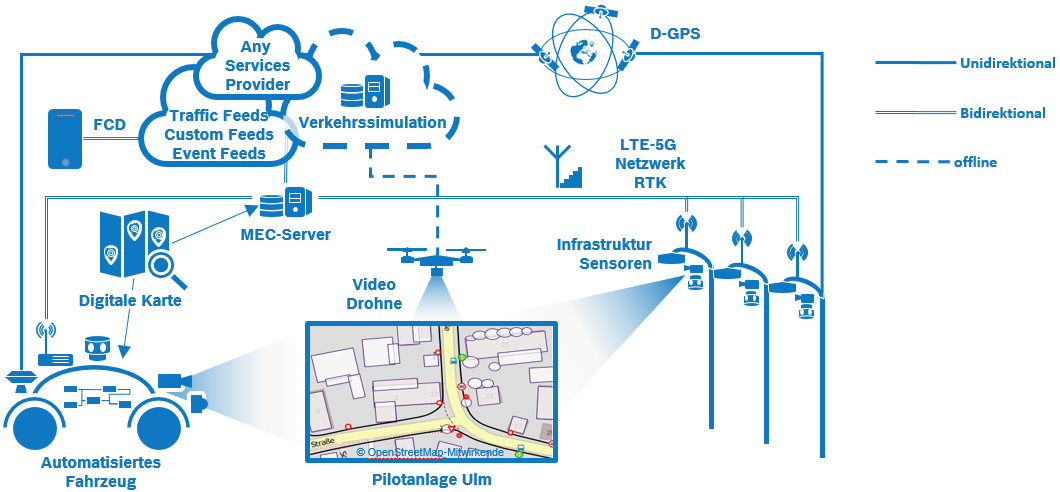
\includegraphics[width=0.7\linewidth]{resources/img/mec_view_arch}
\caption[Überblick MEC-View Projekt]{Überblick MEC-View Projekt \cite[]{mecViewWeb}}
\label{fig:intro_mec_view_arch}
\end{figure}

In urbanen Gebieten
sollen neben Daten von fahrzeuginternen Sensoren auch Informationen externer Infrastruktur-Sensoren verwendet werden,
damit autonome Fahrzeuge eine fundierte Verhaltensentscheidung auf Basis eines detaillierten Umfeldmodells treffen können.
Im Rahmen des Forschungsprojektes MEC-View wird eine Pilot-Anlage zur Umfelderfassung an einer vorfahrtberechtigten Straßenkreuzung
in Ulm aufgebaut und getestet. In dieser Anlage werden die Verkehrsteilnehmer über Kameras und LIDAR-Sensoren erfasst
und die ermittelten Daten über ein schnelles LTE/5G-Mobilfunknetz an einen \textit{Mobile Edge Computing} (\acrshort*{mec}) Server übertragen.
Hier werden die Daten in Echtzeit zu einem Umfeldmodell fusioniert, welches anschließend den autonomen Fahrzeugen
zur besseren Navigation zur Verfügung gestellt wird. Beteiligt an diesem Forschungsprojekt sind neben
der IT-Designers GmbH unter anderem auch die Daimler AG, die Robert Bosch GmbH, Osram, Nokia und die Universität Ulm.
Jeder Projektpartner ist verantwortlich für unterschiedliche Teilaspekte des Projektes. Die IT-Designers GmbH,
bei welcher diese Arbeit angefertigt wird, entwickelt den MEC-Server und ist verantwortlich für das
Teilprojekt \textit{Luftbeobachtung}. \cite[]{mecViewWeb}

\subsection{Das MEC-View Teilprojekt Luftbeobachtung}
\label{sec:mecview_sim}

Im MEC-View Teilprojekt \textit{Luftbeobachtung} werden Verkehrsanalysen und Simulationen erstellt, welche dabei helfen
das Verhalten des Verkehrs besser zu verstehen und es somit ermöglichen, diesen zu optimieren.
Mithilfe der Analysen kann beispielsweise untersucht werden, wie durch die Anpassung von Verkehrssteuerungsanlagen
oder durch die Änderung des Fahrverhaltens einzelner Fahrzeuge, eine Verbesserung der Verkehrssituation erreicht werden kann.
Die Erkenntnisse können insbesondere auch in die Verhaltenssteuerung von autonomen Fahrzeugen mit einfließen.
Aus diesem Grund sind entsprechende Untersuchungen auch für das MEC-View Hauptprojekt relevant.

Die Untersuchungen werden im MEC-View Projekt anhand von Luftbeobachtungen durchgeführt, welche von Drohnen getätigt werden.
In den Videoaufnahmen werden mithilfe eines neuronalen Netzes die Positionen und Fahrzeugklassen der Verkehrsteilnehmer ermittelt.
Mittels dieser kann anschließend beispielsweise die Geschwindigkeit und Beschleunigung der einzelnen Fahrzeuge bestimmt werden.
Zur Erstellung der Analysen ist es zudem wichtig, eine Kenntnis der Topologie der untersuchten Straßen, das heißt des
Verlaufs der Fahrbahnen und Spuren, zu besitzen. In Kombination mit den Fahrzeugpositionen können so interessante
Kenngrößen wie der Verkehrsfluss oder die Verkehrsdichte ermittelt werden.

\section{Motivation und Ziele}
\label{sec:motivation_goals}

Im Rahmen dieser Arbeit wird ein Verfahren zur automatischen Erkennung von Fahrspuren in Luftaufnahmen
auf Basis von Trajektoriedaten entwickelt. Die Spurerkennung wird in die Anwendung \textit{Vehicle-Tracker}
integriert, welche im Rahmen des MEC-View Luftbeobachtungs Projekt erstellt wird. Sie dient der Auswertung
von Luftbeobachtungen des Straßenverkehrs.
In der \textit{Vehicle-Tracker} Applikation mussten bislang die Fahrspurverläufe in jeder Aufnahme
händisch definiert werden. Dieser Prozess ist insbesondere dann aufwendig, wenn die zu untersuchenden
Straßenabschnitte beispielsweise mehrspurige Kreuzungen oder Kreisverkehre beinhalten. Das in dieser Arbeit
entwickelte Spurerkennungs-Modul soll die manuelle Spur-Definition weitestgehend ersetzen und es so ermöglichen
in Zukunft mehr Luftaufnahmen mit weniger Aufwand auszuwerten.

Der Verlauf und die Geometrie der Fahrspuren wird in dieser Thesis anhand der Bewegungsbahnen von Fahrzeugen, den sogenannten Trajektorien,
ermittelt. Im Gegensatz zu einer visuellen Detektierung hat das Verfahren den Vorteil, dass Fahrspuren auch in Aufnahmen
mit schlechten Lichtverhältnissen oder Verdeckungen der Fahrbahnen und Spurmarkierungen erkannt werden können.

Zum Thema Spurerkennung existieren zwar bereits Veröffentlichungen (siehe Abschnitt \ref{sec:rw_lane_detection}),
allerdings können die
vorgestellten Methoden meist nur in sehr speziellen Szenarien eingesetzt werden oder die erkannten Spuren
entsprechen den realen Fahrspurverläufen nur schlecht. Ziel dieser Arbeit ist es, ein Verfahren zu entwickeln,
welches Fahrspuren in möglichst vielen unterschiedlichen Szenarien erkennen kann.
Die Spuren sollen außerdem den realen Fahrbahnverläufen so gut wie möglich entsprechen.

\section{Aufbau dieser Arbeit}
\label{sec:aufbau}

Die vorliegende Arbeit ist wie folgt strukturiert:

\begin{itemize}
    \item Die zum Verständnis der Arbeit und des entwickelten Spurerkennungsalgorithmus benötigten
            Grundlagen sind in \textbf{Kapitel \ref{sec:position_extraction} und \ref{sec:tra_clustering}} beschrieben.
            Kapitel \ref{sec:position_extraction} erläutert, wie aus Luftaufnahmen die Trajektorien von Fahrzeugen
            rekonstruiert und in ein Weltkoordinatensystem überführt werden können.
            Kapitel \ref{sec:tra_clustering} stellt die grundlegenden Konzepte der Clusteranalyse vor, welche
            bei der Umsetzung der Spurerkennung zum Einsatz kommt.
    \item In \textbf{Kapitel \ref{cha:related_work}} werden verwandte Arbeiten, welche sich bereits mit
            der Thematik der Spurerkennung und der Clusteranalyse von Trajektorien befassen, vorgestellt und untersucht.
            Zudem werden Defizite der vorhandenen Lösungen und benötigte Neuerungen aufgezeigt.
    \item In \textbf{Kapitel \ref{cha:konzeption}} wird das Konzept für die Umsetzung der Spurerkennung vorgestellt.
            Es werden Anforderungen definiert und das Spurerkennungs-Modul wird in den Gesamtkontext
            der Applikation \textit{Vehicle-Tracker} eingeordnet.
    \item Nach der Konzeption wird in \textbf{Kapitel \ref{cha:realisation}} erläutert, wie die Spurerkennung in dieser Arbeit
            umgesetzt wurde. Es werden die verschiedenen Schritte des entwickelten Algorithmus vorgestellt.
    \item In \textbf{Kapitel \ref{cha:results}} wird der Spurerkennungsalgorithmus evaluiert.
            Es wird auf die Stärken und Schwächen der wichtigsten Verarbeitungsschritte des Algorithmus eingegangen.
            Außerdem werden konkrete Ergebnisse in Form von Screenshots der erkannten Fahrspuren vorgestellt.
    \item \textbf{Kapitel \ref{cha:end}} bildet den Schluss dieser Masterarbeit. Hier werden die Ergebnisse der
            Arbeit nochmals zusammengefasst und es wird ein Ausblick gegeben, in welchen Anwendungsgebieten die Spurerkennung
            in Zukunft eingesetzt werden kann und welche Verbesserungen an dem entwickelten Verfahren noch vorgenommen werden können.
    \item Im \textbf{\hyperref[cha:anhang_a]{Anhang}} dieser Arbeit sind Aufnahmen der Straßenabschnitte dargestellt,
            mit deren Hilfe der Spurerkennungsalgorithmus entwickelt und evaluiert wurde.
\end{itemize}



% % %%%%%% Literaturverzeichnis (darf im deutschen nicht in den Anhang!)
% Einfaches Literaturverzeichnis
% \input{chapters/bibEinfach}
% Literaturverzeichnis mit Bibtex
\bibliography{bib/sources}

\printglossary

% % %%%%%% Anhang
\appendix
% %!TEX root = ../Thesis.tex

\chapter{Anhang - Verwendete Datensätze}
\label{cha:anhang_a}

Nachfolgend sind Aufnahmen der in dieser Arbeit verwendeten Luftaufnahmen zu sehen.

\subsection*{Datensatz Entennest}

\begin{figure}[H]
\centering
    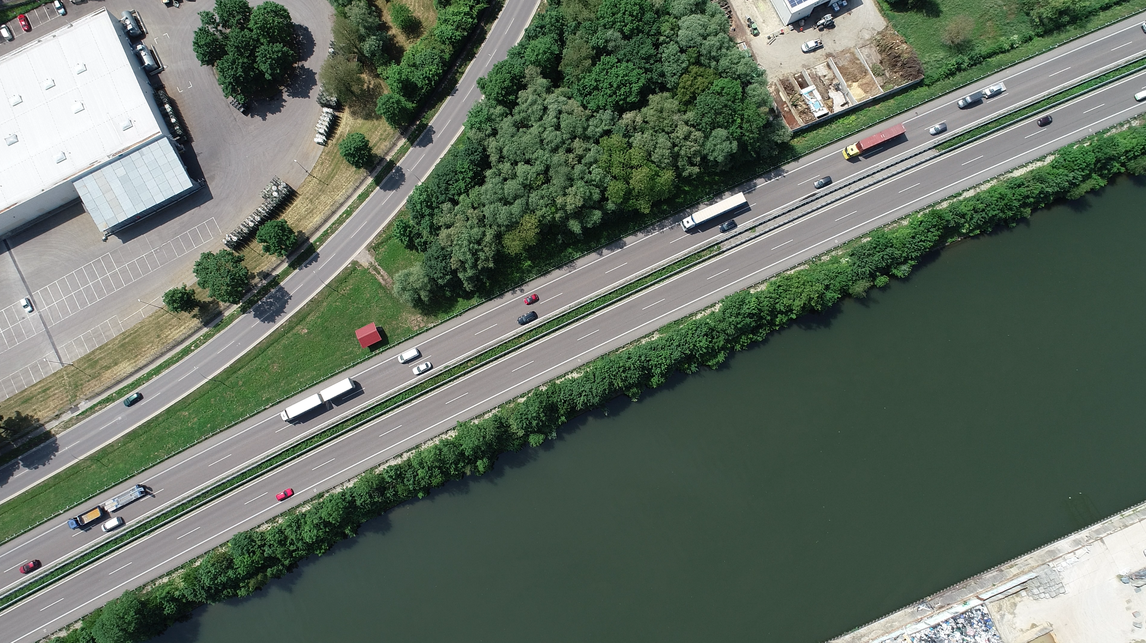
\includegraphics[width=0.6\linewidth]{resources/img/Anhang/Entennest}
\caption{Staßenabschnitt Aufnahme Entennest}
\label{fig:anhang_ds_entennest}
\end{figure}

\subsection*{Datensatz Neckartor}

\begin{figure}[H]
\centering
    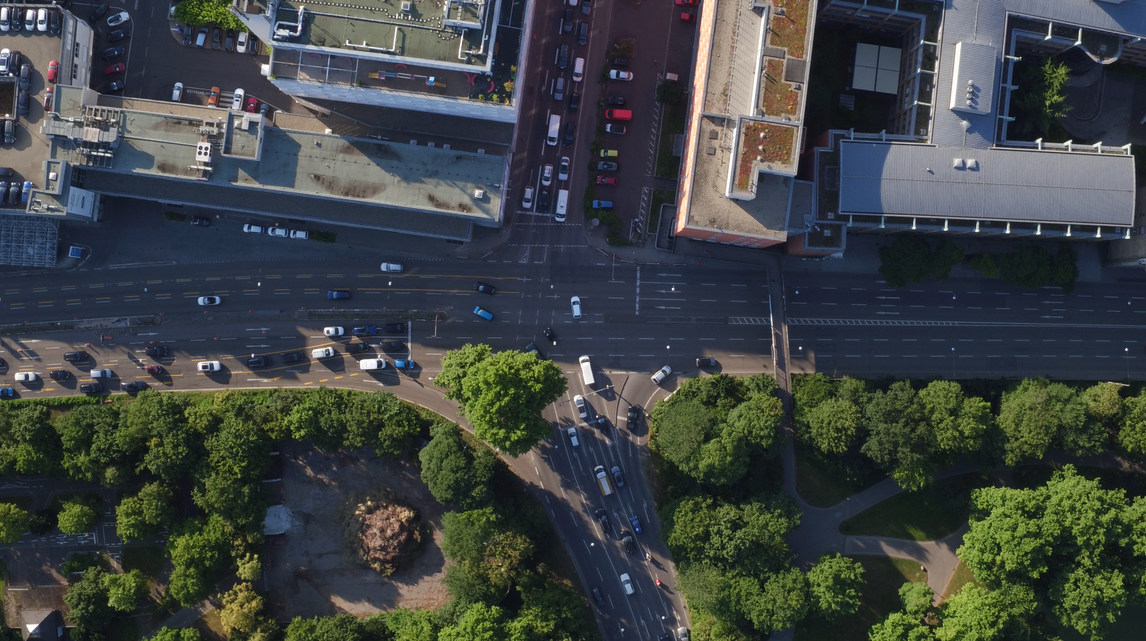
\includegraphics[width=0.6\linewidth]{resources/img/Anhang/Neckartor}
\caption{Staßenabschnitt Aufnahme Neckartor}
\label{fig:anhang_ds_neckartor}
\end{figure}

\subsection*{Datensatz Heilbronner-Straße}

\begin{figure}[H]
\centering
    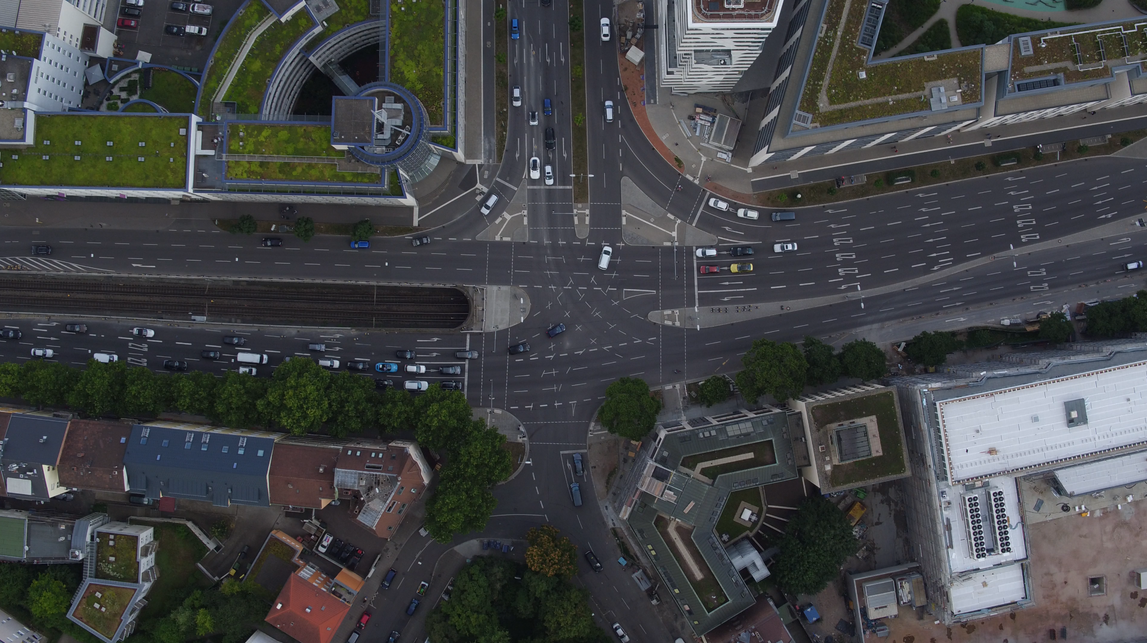
\includegraphics[width=0.6\linewidth]{resources/img/Anhang/Heilbronner}
\caption{Staßenabschnitt Aufnahme Heilbronner-Straße}
\label{fig:anhang_ds_heilbronner}
\end{figure}

\subsection*{Datensatz Düsseldorf}

\begin{figure}[H]
\centering
    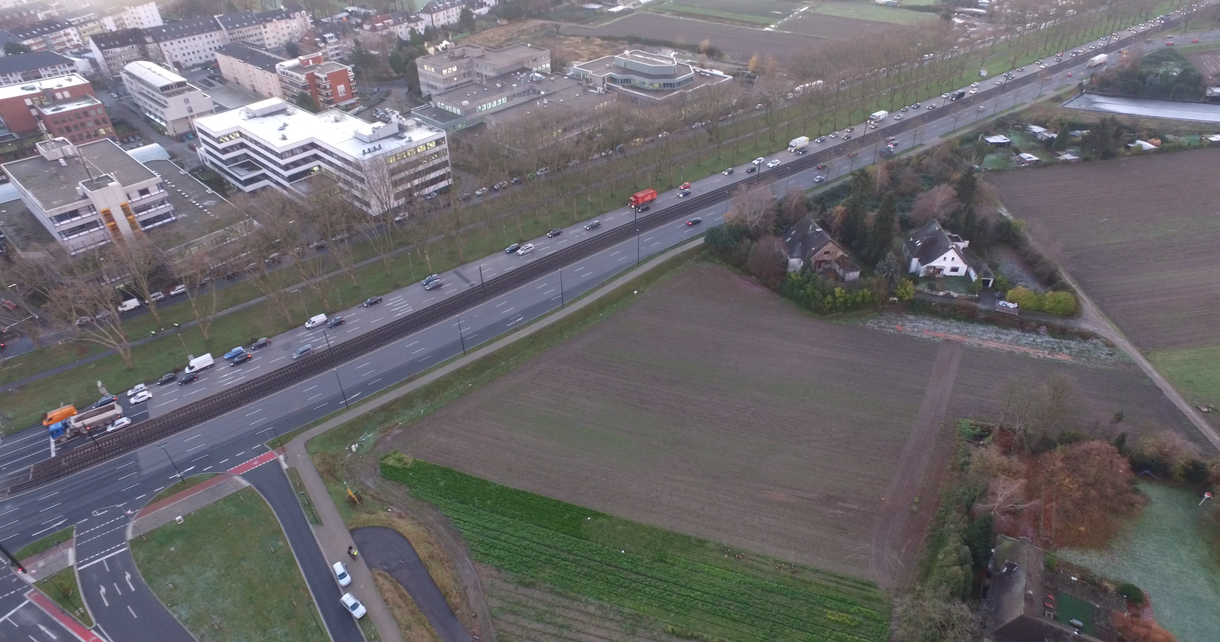
\includegraphics[width=0.6\linewidth]{resources/img/Anhang/Duesseldorf}
\caption{Staßenabschnitt Aufnahme Düsseldorf}
\label{fig:anhang_ds_duesseldorf}
\end{figure}

\subsection*{Datensatz Steinheim}

\begin{figure}[H]
\centering
    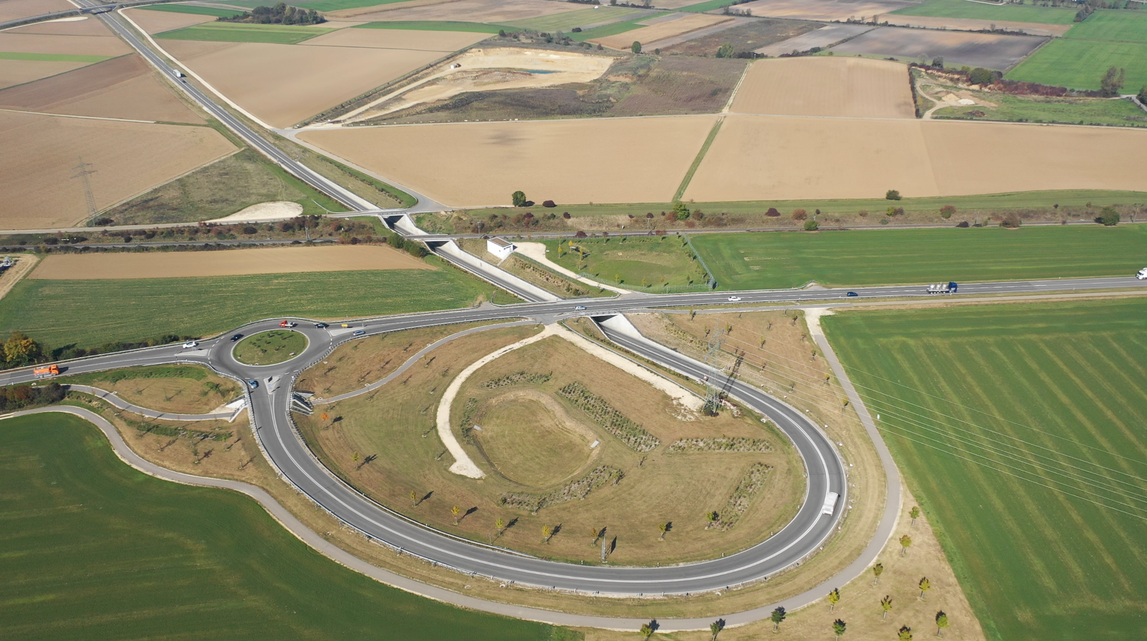
\includegraphics[width=0.6\linewidth]{resources/img/Anhang/Steinheim}
\caption{Staßenabschnitt Aufnahme Steinheim}
\label{fig:anhang_ds_steinheim}
\end{figure}

% %  Inhalt ENDE %%%%%%%%%%%%%%%%%%%%%%%%%%%%%%%%%%%%%%%%%%%%%%%%%%%%%%%%%%
\end{document}
